\documentclass[letterpaper]{article}
\usepackage{isea}
\usepackage[pdftex]{graphicx}
\usepackage{times}
\usepackage{helvet}
\usepackage{courier}
\usepackage{svg}
\usepackage[numbers]{natbib}
\usepackage{url}
\pdfinfo{
  /Title (DSA switches: domesticating a savage beast)
  /Author (Vladimir Oltean)}
\title{DSA switches: domesticating a savage beast}
\author{Vladimir Oltean\\
  \\vladimir.oltean@nxp.com\\
}
\setcounter{secnumdepth}{0}

\begin{document}
\maketitle
\begin{abstract}

  The DSA subsystem was originally built around Marvell devices, but has since
  been extended to cover a wide variety of hardware with even wider views of
  their management model. This paper uses the DSA architecture overview
  \cite{dsa-netdev-2.1} as a primary source and discusses the changes in DSA
  that took place in the last years for this wide variety of switches to offer
  more services, and in a more uniform way, to the larger network stack.

  Summarized, these changes are:

\begin{itemize}
\item Acknowledging switches which only have DSA tags for control plane
      packets, and modifying the bridge driver to accept termination of data
      plane packets from these switches.
\item Support for unoffloaded upper interfaces.
\item Support for more cross-chip topologies than the basic daisy chain, while
      maintaining the basic principle that network interfaces under the same
      bridge can forward from one to another, and interfaces under different
      bridges don't.
\end{itemize}

\end{abstract}

\section{Keywords}

DSA, bridge, switchdev, offloading, cross-chip bridging, imprecise RX, TX
forwarding offload, RX filtering.

\section{The data plane and the control plane}

The original DSA architecture, seen in figure \ref{dsa-overview}, has remained
unchanged to this day. It stipulates that one virtual network interface should
be exposed for each front-facing switch port, and no virtual network interface
should be exposed for the ports facing inwards (CPU ports, DSA/cascade ports).
DSA network interfaces should not only be conduit interfaces for retrieving
ethtool statistics and registering with the PHY library, but they should be
fully capable of sending and receiving packets. This is accomplished via the
DSA tagging protocol drivers, which are hooks in the RX and TX path of the host
Ethernet controller (the DSA master) which multiplex and demultiplex packets
to/from the correct virtual switch interface based on switch-specific metadata
that is placed in the packets.

\begin{figure}[ht]
  \centering
  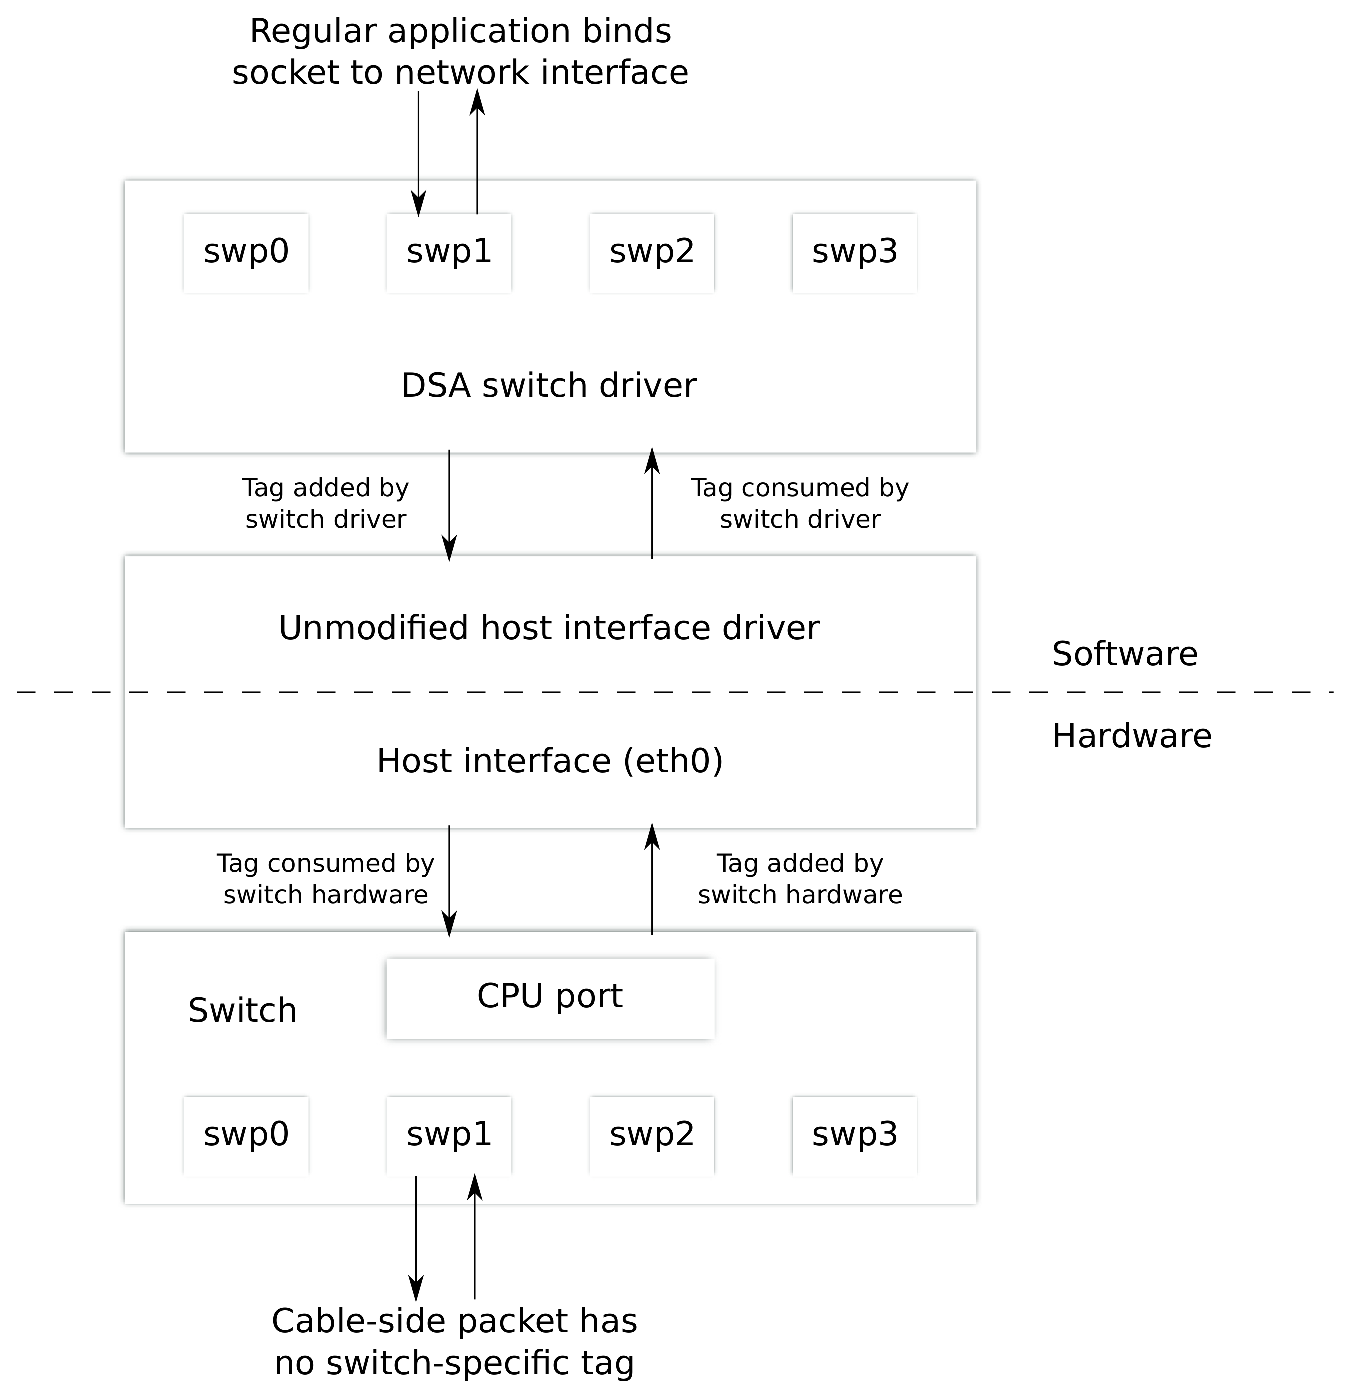
\includegraphics[width=\columnwidth]{dsa-overview.eps}
  \caption{Overview of packet flow with DSA switches}
  \label{dsa-overview}
\end{figure}

In this model, the basic function of a network switch from a hardware
designer's perspective, which is to switch packets, is an optional feature from
the Linux network stack's perspective, and was added years after the original
design had been established. This is one of the first major hurdle software
engineers need to get over when starting development in this area: DSA is not
simply a switch driver, it is a networking driver framework, which first and
foremost needs to cater to the most basic network connectivity needs, and which
has optional hardware acceleration features.

Behind the seemingly uniform implementation of DSA tagging protocols and switch
drivers, which are tightly managed by the DSA framework, lie many differences
and subtleties that make the feature set exposed by two different DSA switches
to the network stack very different.

The majority of network switches capable of management have some sort of
distinction between the data plane packets and the control packets. These
different flows, detailed in figure \ref{dsa-control-plane-vs-data-plane} as
well as below, are superimposed on top of the same hardware ports. For this
reason, even if control and data packets travel through the same Ethernet
ports, it may be helpful to visualize them three dimensionally to understand
the key differences.

\begin{figure}[ht]
  \centering
  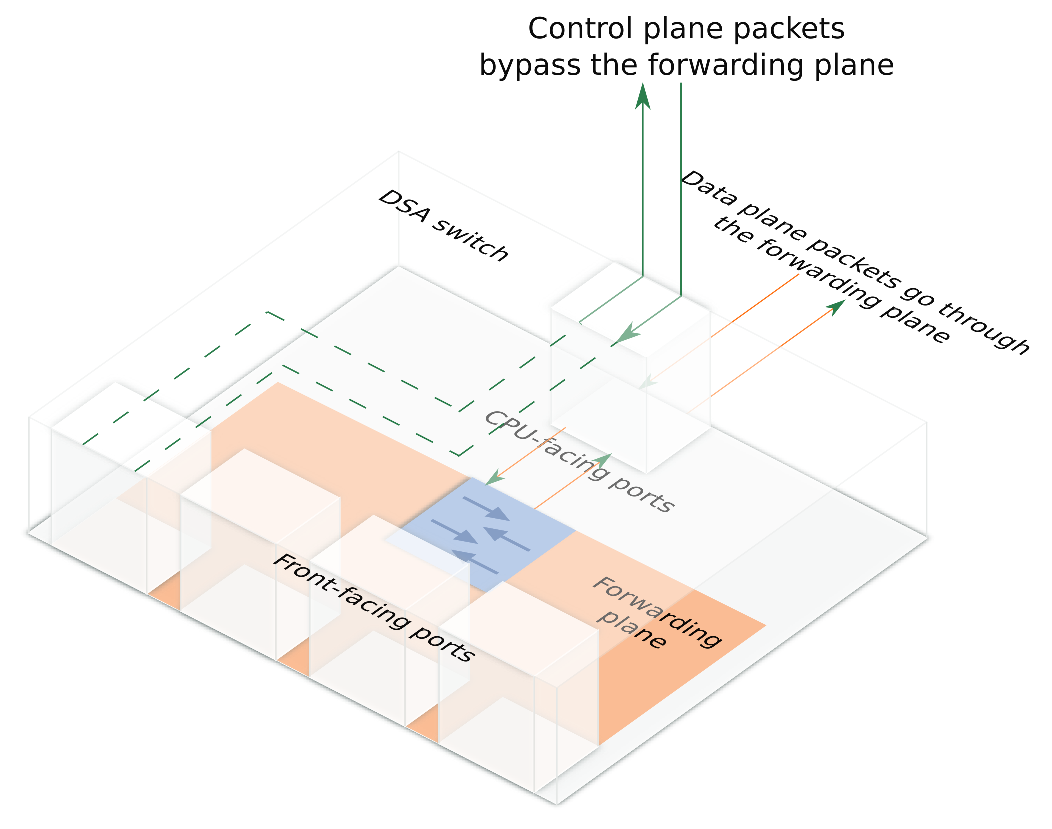
\includegraphics[width=\columnwidth]{dsa-control-plane-vs-data-plane.eps}
  \caption{DSA control plane vs data plane}
  \label{dsa-control-plane-vs-data-plane}
\end{figure}

At the most basic level, control packets, which must be used for link-layer
control protocols like STP, PTP, EAP, have the ability to target a specific
egress port and to override its STP state (inject into a BLOCKING port). These
packets typically bypass the forwarding layer of the switch and the frame
analysis stage of the ingress (CPU) port and are injected directly into the
egress port. The implications are that metadata such as QoS class and VLAN ID
must be specified by the operating system driver directly as part of the DSA
tag, and that hardware address learning is not performed on the CPU port.

On the opposite side of the spectrum, data plane packets do not perform STP
state override, are subject to hardware address learning on the CPU port, but
also cannot be steered towards a precise destination port, since they are also
subject to the forwarding rules of the switch. The format of these packets
might vary from a special bit in the DSA tag which marks them as subject to
forwarding, to the complete absence of a DSA tag. For these packets, the CPU
port acts like any other bridge port.

At the extreme, there exists a \verb|DSA_TAG_PROTO_NONE| tagging protocol,
which admits defeat and does not attempt to multiplex/demultiplex virtual
switch interfaces from the DSA tag, and all network I/O through such a switch
takes place through the DSA master which is seen as a switched endpoint. The
network interfaces registered for the switches are only used for control
operations (ethtool, PHY library) and are "dead" to the network stack both for
control plane and for data plane packets. These are the "unmanaged" switches.

Finally, in some switch designs, injecting a control packet is an expensive
operation which cannot be sustained at line rate, and the bulk of the traffic
(the data plane packets) should be injected, from the hardware designer's
perspective, directly through the DSA master interface, with no DSA tag.
These are the "lightly managed" switches, and their virtual DSA interfaces are
similarly "dead" to the network stack except for link-local packets.

The most basic and common approach with this type of hardware is to simply set
up a user space configuration to perform the traffic termination from the
switching domain on the DSA master itself. For some packets to target a single
switch port, the user is required to install a bridge VLAN on the switch port
which is egress-tagged towards the CPU port, then create an 8021q upper with
the same VLAN ID on top of the DSA master, and send/receive traffic through the
8021q upper of the DSA master. This approach is, however, undesirable for two
reasons. First, \verb|DSA_TAG_PROTO_NONE| is the only tagging protocol which
needs special treatment from user space, which hurts the DSA framework's goal
in exposing a uniform set of commands for user interaction. Second, it is
inherently impossibile to run control protocols for this switch - that would
fundamentally require a tagging protocol which is not \verb|DSA_TAG_PROTO_NONE|.
Attempting to fix that, and making the switch network interfaces be capable of
traffic but only for control protocols, by creating a specific tagging protocol
which behaves as \verb|DSA_TAG_PROTO_NONE| for data packets, creates yet
another road block: bridging DSA interfaces with non-DSA (foreign) interfaces
is impossible, which is an important use case for boards with a switch and a
Wi-Fi AP (home routers). Interfaces that are DSA masters cannot be added to a
bridge either (they can only as long as they use \verb|DSA_TAG_PROTO_NONE|
\cite{reject-dsa-masters-as-bridge-ports}).

A slightly better integrated way of achieving the same result is the relatively
new software-defined DSA tagging protocol named \verb|tag_8021q|, which can
bring both the lightly managed and unmanaged switches closer to the user model
exposed by DSA switches with hardware support for a DSA tagging protocol.

The \verb|tag_8021q| protocol is fundamentally still sending data plane packets
from the perspective of the hardware, so there are things it cannot accomplish,
like STP state override. Therefore, \verb|tag_8021q| must always be augmented
by switch-specific methods of injecting and extracting control packets in order
to offer full functionality, and for this reason, this tagging protocol is
offered as library code and not a full drop-in solution. Additionally, the DSA
framework has traditionally not enforced any meaningful distinction between
data plane and control plane packets, since originally, the assumption was that
all packets injected by the software network stack should be control packets.

To unify the hardware and the software notions, and to use these chips in the
way they were meant to, the network stack must be taught about data plane
packets. The \verb|tag_8021q| model breaks down when DSA switch interfaces
offload a VLAN-aware bridge, which is in fact their primary use cases. This is
because the source port of the switch cannot be retrieved based on the VLAN ID
by the tagging protocol driver on RX, because the VLANs are under the control
of the bridge driver, not DSA, and there is no guarantee that a VLAN is
uniquely installed on a single switch port. So bridging with foreign interfaces
becomes equally impossible.

The decisive changes which made these switches correctly offload a VLAN-aware
bridge come in the form of not attempting to report a precise source port on RX
for data plane packets, just a plausible/imprecise one. As long as some
requirements inside the software bridge's ingress path are satisfied (valid STP
state, VLAN ID from the packet is in the port's membership list), the bridge is
happy to accept the packet as valid, and process it on behalf of the imprecise
DSA interface that was reported.

Complications arise due to the fact that the software bridge might learn the
MAC SA of these packets on a potentially wrong port, and deliver those packets
on the return path towards the wrong port. Additionally, due to bandwidth
constraints, DSA interfaces do not synchronize their hardware FDB with the FDB
of the software bridge, so the software bridge does not have an opportunity to
figure out the real source port of imprecise packets.

To give DSA the chance to right a wrong, the bridge driver was modified to
support TX forwarding offload \cite{bridge-tx-fwd-offload}. With this feature,
the software bridge avoids cloning an skb which needs to be flooded to multiple
ports, and sends only one copy of the packet towards a single network interface
from each "hardware domain" that the flooded packet must reach. The port driver
is responsible with looking up its hardware FDB for that packet and replicate
the packet as needed.  This is a useful feature in itself, because with
switches with a large port count, multicast traffic on the bottlenecked link
between the DSA master and the CPU port is reduced, and packets are replicated
inside the hardware.  But with the lightly-managed and unmanaged switches, it
makes the imprecise RX work correctly, since the TX is also imprecise. So even
though the software bridge did learn the MAC SA of the packets on the wrong
source port, that source port is in the same hardware domain with the right
port, and even though the software FDB is incorrect, the hardware FDB isn't. So
DSA drivers for lightly-managed and unmanaged switches have a chance to
properly terminate traffic on behalf of a VLAN-aware bridge, in a way that is
compatible with bridging with foreign interfaces, and with a user space
interaction procedure that is much more uniform with DSA drivers that always
send and receive packets with a DSA tag.

\section{Unoffloaded software upper interfaces}

Support for unoffloaded upper interfaces running on top of DSA switch ports,
such as the bridge, VLAN, macvlan, bonding interfaces, has always been baked
into DSA's core architecture. Surely, it came at a high cost, which is to not
use the hardware to its full potential. However, this feature got broken when
switchdev was created and DSA was integrated with it in order to offer hardware
offload for the Linux bridge. This section details the changes made to
switchdev in order for DSA to regain this functionality.

Recently, DSA has also gained support for offloading other virtual network
interfaces than the Linux bridge. These are the hsr driver (which supports the
HSR and PRP industrial redundancy protocols) \cite{dsa-hsr} and the
bonding/team drivers (which support the link aggregation protocol)
\cite{dsa-lag}.

Not all switches are capable of offloading hsr and team/bonding, and DSA's
policy is to fall back to a software implementation when hardware offload
cannot be achieved: the bandwidth to/from the CPU is often times good enough
that this is not impractical.

However, DSA's policy could not be enforced right away with the expected
results, due to two roadblocks that led to further changes in the kernel code
base.

To not offload an upper interface means for DSA that the physical port should
behave exactly as it would if it was a standalone interface with no switching
to the others except the CPU port, and which is capable of IP termination.

But when the unoffloaded upper interface (the software LAG) is part of a
bridge, the bridge driver makes the incorrect assumption that it is capable of
hardware forwarding towards all other ports which report the same physical
switch ID. Instead, forwarding to/from a software LAG should take place in
software. This has led to a redesign of the switchdev API, in that drivers must
now explicitly mark to the bridge the network interfaces that are capable of
autonomous forwarding \cite{switchdev-explicit-offloading-api}; the new default
being that they aren't. In the new model, even if two interfaces report the
same physical switch ID, they might yet not be part of the same hardware domain
for autonomous forwarding as far as the bridge is concerned.

The second roadblock, even after the bridge was taught to allow software
forwarding between some interfaces which have the same physical switch ID, was
FDB isolation in DSA switches. Up until this point, the vast majority of DSA
drivers, as well as the DSA core, have considered that it is enough to offload
multiple bridges by enforcing a separation between the ports of one bridge and
the ports of another at the forwarding level. This works as long as the same
MAC address (or MAC+VLAN pair, in VLAN-aware bridges) is not present in more
than one bridging domain at the same time. This is an apparently reasonable
restriction that should never be seen in real life, so no precautions have been
taken against it in drivers or the core.

\begin{figure}[ht]
  \centering
  \includegraphics[width=\columnwidth]{dsa-need-for-fdb-isolation.eps}
  \caption{Pinging between two stations connected by DSA using software forwarding}
  \label{dsa-need-for-fdb-isolation}
\end{figure}

The issue, described in figure \ref{dsa-need-for-fdb-isolation}, is that a DSA switch is still a switch, and for every packet it
forwards, regardless of whether it is received on a standalone port, a port
under a VLAN-unaware bridge or under a VLAN-aware one, it will attempt to look
up the FDB to find the destination. With unoffloaded LAGs on top of a
standalone DSA port, where forwarding between the switched domain and the
standalone port takes place in software, the expectation that a MAC address is
only present in one bridging domain is no longer true. From the perspective of
the ports under the hardware bridge, a MAC address might come from the outside
world, whereas from the perspective of the standalone ports, the same MAC
address might come from the CPU port. So without FDB isolation (which is a
hardware-specific mechanism by which FDB lookups performed on a source port are
made to not match on FDB entries pointing towards a port that is not in the
same hardware forwarding domain), the standalone port might look up the FDB for
a MAC address and see that it could forward the packet directly to the port in
the hardware bridge domain, where that packet was learned by the bridge port,
shortcircuiting the CPU. But the forwarding isolation rules put in place will
prevent this from happening, so packets will be dropped instead of being
forwarded in software.

Individual drivers have started receiving patches for FDB isolation between
standalone ports and bridged ports, but it is possible to conceive real life
situations where even FDB isolation between one bridge and another must be
maintained. Since the DSA core, at the time of writing, does not enforce FDB
isolation through its API and many drivers already have been written without it
in mind, it is to be expected that many years pass until DSA drivers offer a
uniform set of services to upper layers in this regard. Even with the core DSA
framework in place, driver writers still are responsible for finding (sometimes
creative) ways of isolating FDB lookups between ports that are standalone and
ports that are members of a bridge, as well as between ports that are members
of different bridges. The solutions can vary between cropping a range of VLAN
IDs to be used for isolating VLAN-unaware bridges, and restricting the user to
only create a single VLAN-aware bridge if VLANs of one bridge cannot be
isolated from VLANs of another, to using hardware specific Filtering
Identifiers (FID) which remap the same VLAN IDs from packets to different
internal VLAN structures from the 4K space, depending on the bridging domain
they belong to, to remapping VLANs to an internal space larger than 4K.

\section{RX filtering}

In the context of DSA, RX filtering refers to the technique of teaching
switches which addresses must be filtered towards the host and delivered to the
CPU ports. There are multiple possible ways to force a certain \{MAC DA, VLAN
ID\} pair to be sent towards the CPU, either by installing an FDB entry in
hardware, or by installing an ACL rule if the switch has a programmable TCAM.

Even if no such thing as a MAC address for a switch port exists, DSA network
interfaces have MAC addresses of their own, since they are also capable of
termination, not just forwarding. By default, that MAC address is inherited
from the DSA master's MAC address, with an option to override the address of
each port from other sources like the device tree. Traditionally, DSA has not
configured the switches in any way so as to make sure that packets destined
towards the switch ports' addresses, or the DSA master's address, or a bridge
upper interface's address, are really filtered only towards the host.

The end result varies depending on the exact hardware switch implementation,
but the typical case is that of a fully managed switch, whose tagging driver
sends only control packets. If the switch is configured to not perform hardware
address learning for the MAC SA from those control packets, or if it outright
cannot do it, then rules that match on host addresses are simply absent from
hardware. Therefore, the packets destined for the host are reaching it via
flooding. The host is not the only flooding destination however, however, these
packets are flooded towards all other ports that are in the same bridging
domain with the ingress port. There was a desire to change this behavior.

It turns out that addresses corresponding to interfaces on the host are not the
only addresses that the switch must send to the CPU via a non-flooding based
mechanism. There are many kinds of use cases where DSA switch ports are in a
bridging domain with "foreign" (non-DSA) interfaces. A typical example is a
Wi-Fi AP interface, which is in the same bridging domain with a DSA switch that
handles the LAN ports. This topology can be seen in many home Wi-Fi routers
running OpenWRT. Here, the effects of not having hardware address learning on
the CPU port can be much more disastrous \cite{switchdev-fdb-on-foreign-interfaces}.
The root of the Wi-Fi roaming issue can be summarized as follows: if a station
used to be learned by the switch on a certain port, but then migrates to
another port which is in the switch's blind spot (such as behind the CPU, where
no hardware address learning takes place), then the stale address will cause
packet loss until it expires, and it may take many minutes until it does age
out. There was also a desire to change this behavior.

Furthermore, taking FDB isolation into consideration, standalone ports (ports
not offloading any interface) should be placed by drivers in a hardware FDB
partition where no learning takes place, and packets are flooded towards their
only possible destination (the CPU port). So there is no immediate need to
implement \verb|IFF_UNICAST_FLT| for standalone ports in DSA, it is only bridge
ports that have a problem.

After gathering all requirements, the conclusion was that the problem needs to
be addressed at the bridge level, and DSA became much tighter integrated with
the software FDB of the bridge, by sniffing for two classes of FDB entries and
offloading them as FDB entries towards its CPU ports:

\begin{itemize}
\item FDB entries learned on foreign interfaces in the same bridging domain as
      a DSA switch interface. This solves the Wi-Fi roaming issue by
      introducing an opt-in "assisted learning on the CPU port" feature which
      replaces the hardware alternative \cite{dsa-assisted-learning}.
\item FDB entries that are local/permanent. The bridge marks the MAC address of
      each bridge port as a local address, and the same goes for the bridge's
      own MAC address. By offloading these entries, packets targeted towards
      the bridge itself are no longer flooded in the entire bridging domain
      \cite{dsa-rx-filtering}.
\end{itemize}

The ultimate goal of RX filtering in DSA is to mark the CPU port as not being
part of the flooding domain of the switch. Ideally, all packets that reach the
host should reach it with a good reason, and not rely on software to drop them
if they are not needed, since this wastes precious CPU cycles. Disabling
flooding towards the CPU (neither unicast nor multicast) is not something
possible today due to several reasons.

A limitation that is still present is the case where the bridge network
interface has upper interfaces of its own (for example an 8021q upper), and
these interfaces do not have the same MAC address as the bridge itself. Since
the bridge driver does not implement \verb|IFF_UNICAST_FLT|, the network stack
will make this interface promiscuous. Packets coming from the hardware DSA side
will still reach this interface via flooding, but with the same limitations as
before. To address this limitation, the \verb|dev_uc_add| API must be extended
to include a VLAN ID as well, then the bridge driver must be modified to
implement \verb|IFF_UNICAST_FLT| and add the MAC addresses of its upper
interfaces as FDB entries that are local/permanent (point towards the bridge).
This way, DSA and other switchdev drivers will receive the information they
need to have a known destination for these virtual interfaces.

Another case in which flooding towards the CPU cannot simply be disabled is
when DSA ports are in a bridge with foreign interfaces. Even if no local
interface needs the packets, a station associated with the Wi-Fi AP might.

\section{Switch topology changes}

Traditionally, the cross-chip setups supported by DSA have been daisy chains,
where all switches except the top-most one lack a dedicated CPU port, and are
simply cascaded towards an upstream switch. There are two new switch topologies
supported by DSA now.

\begin{figure}[ht]
  \centering
  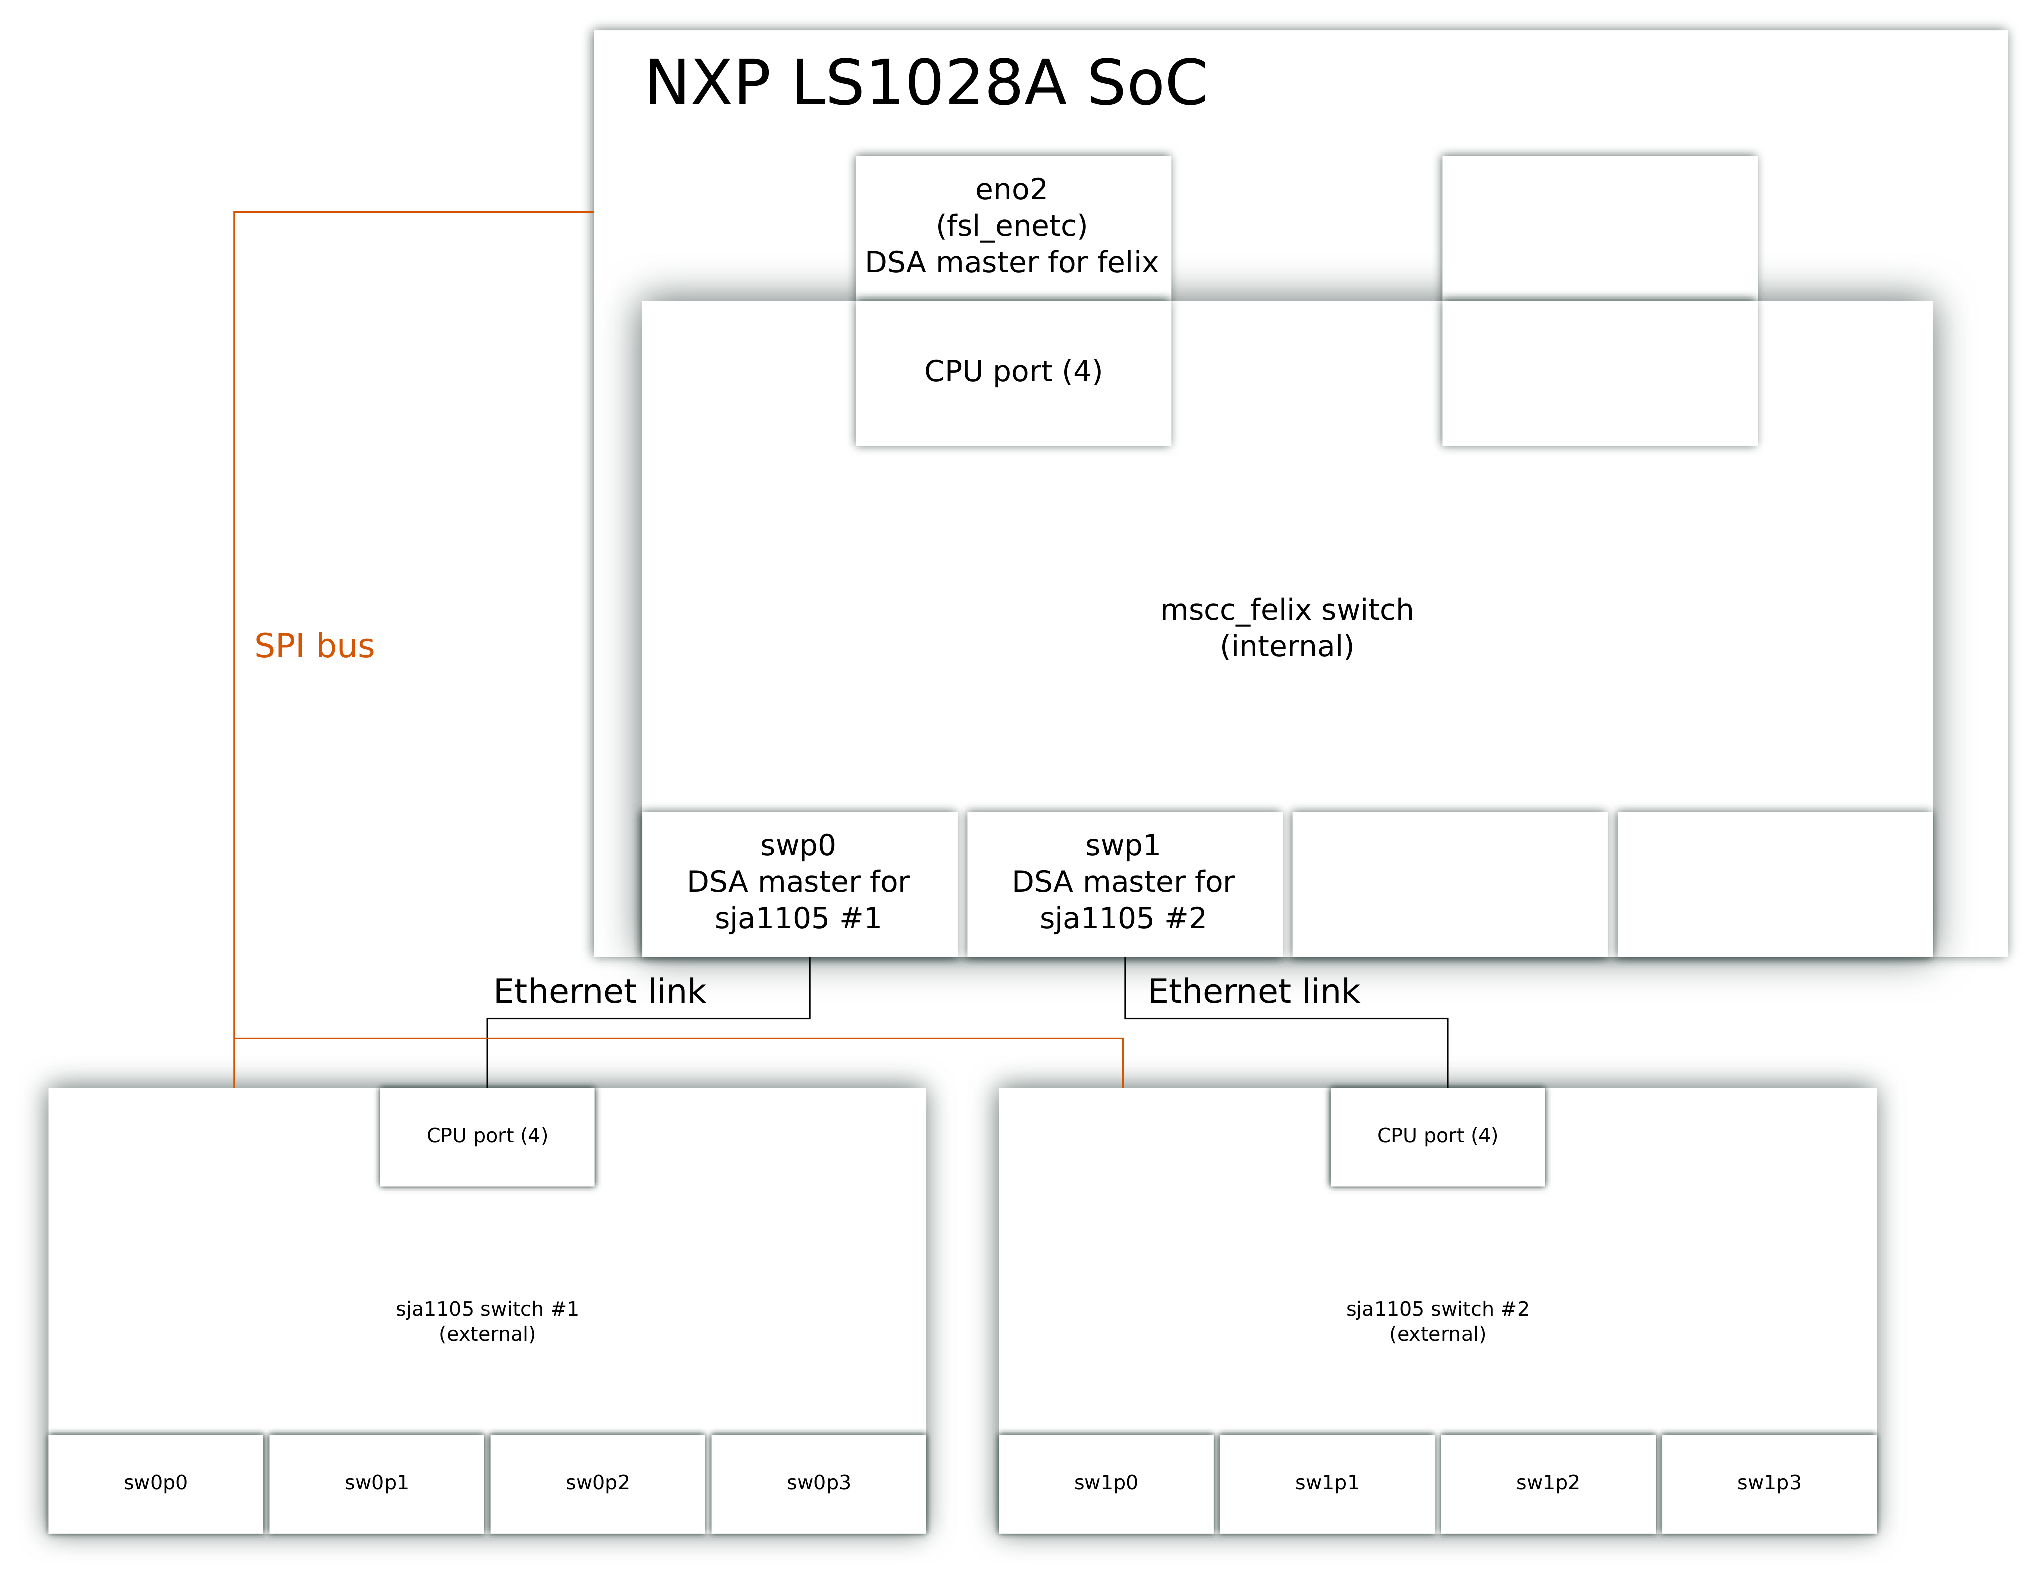
\includegraphics[width=\columnwidth]{felix-sja1105-disjoint-trees.eps}
  \caption{A disjoint tree setup consisting of NXP LS1028A internal switch ports acting as DSA masters for SPI-connected external switches}
  \label{felix-sja1105-disjoint-trees}
\end{figure}

The first is the disjoint tree topology from figure
\ref{felix-sja1105-disjoint-trees}. A DSA tree is comprised of all switches
directly connected to each other which use a compatible tagging protocol (one
switch understands the packets from the other one, and can push/pop them as
needed). Disjoint trees are used when DSA switches are connected to each other,
but their tagging protocols are not compatible.  As opposed to one switch
understanding another's, tag stacking takes place, so in software, more than
one DSA tagging protocol driver needs to be invoked for the same packet. In
such a system, each switch forms its own tree. Disjoint trees were already
supported, but the new changes also permit some hardware forwarding to take
place between switches belonging to different trees. For example, be there an
embedded 5 port DSA switch that has 2 external DSA switches connected to 2 of
its ports. Each embedded DSA switch interface is a DSA master for the external
DSA switch beneath it, and there are 3 DSA disjoint trees in this system. For a
packet to be sent from external switch 1 to external switch 2, it must be
forwarded towards the CPU port. In the most basic configuration, forwarding
between the two external switches can take place in software. However, it is
desirable that the embedded DSA switch that is a master of external switches 1
and 2 can accelerate the forwarding between the two (because the external
switches are tagger-compatible, they are just separated by a switch which isn't
tagger-compatible with them). Under some conditions, this is possible as long
as the embedded DSA switch still has some elementary understanding of the
packets, and can still forward them by MAC DA and optionally VLAN ID, even
though they are DSA-tagged. With the vast majority of DSA tagging protocols,
the MAC DA of the packets is not altered even when a DSA tag is inserted, so
the embedded DSA master can sanely forward packets between one external switch
and another. This is one of the only special cases where DSA master interfaces
can be bridged (they are part of a separate bridge compared to the external
switch ports), because in this case, the DSA masters are part of a bridge with
no software data plane, just a hardware data plane.  The second requirement is
for both the embedded and the external switches to have the same understanding
of what constitutes a data plane packet, and what constitutes a control plane
packet: STP packets received by the external switch should not be flooded by
the embedded switch. Due to the same reason that the embedded switch must still
preserve an elementary understanding of the MAC DA of packets tagged with the
external switch's tagging protocol, this will also be the case, since typical
link-layer protocols have unique link-local multicast MAC addresses.

For this topology, the necessary changes were to permit cross-chip bridging
between ports belonging to different DSA trees, and to allow certain DSA
masters to be bridge ports as long as no software forwarding is required
\cite{dsa-disjoint-trees}.

\begin{figure}[ht]
  \centering
  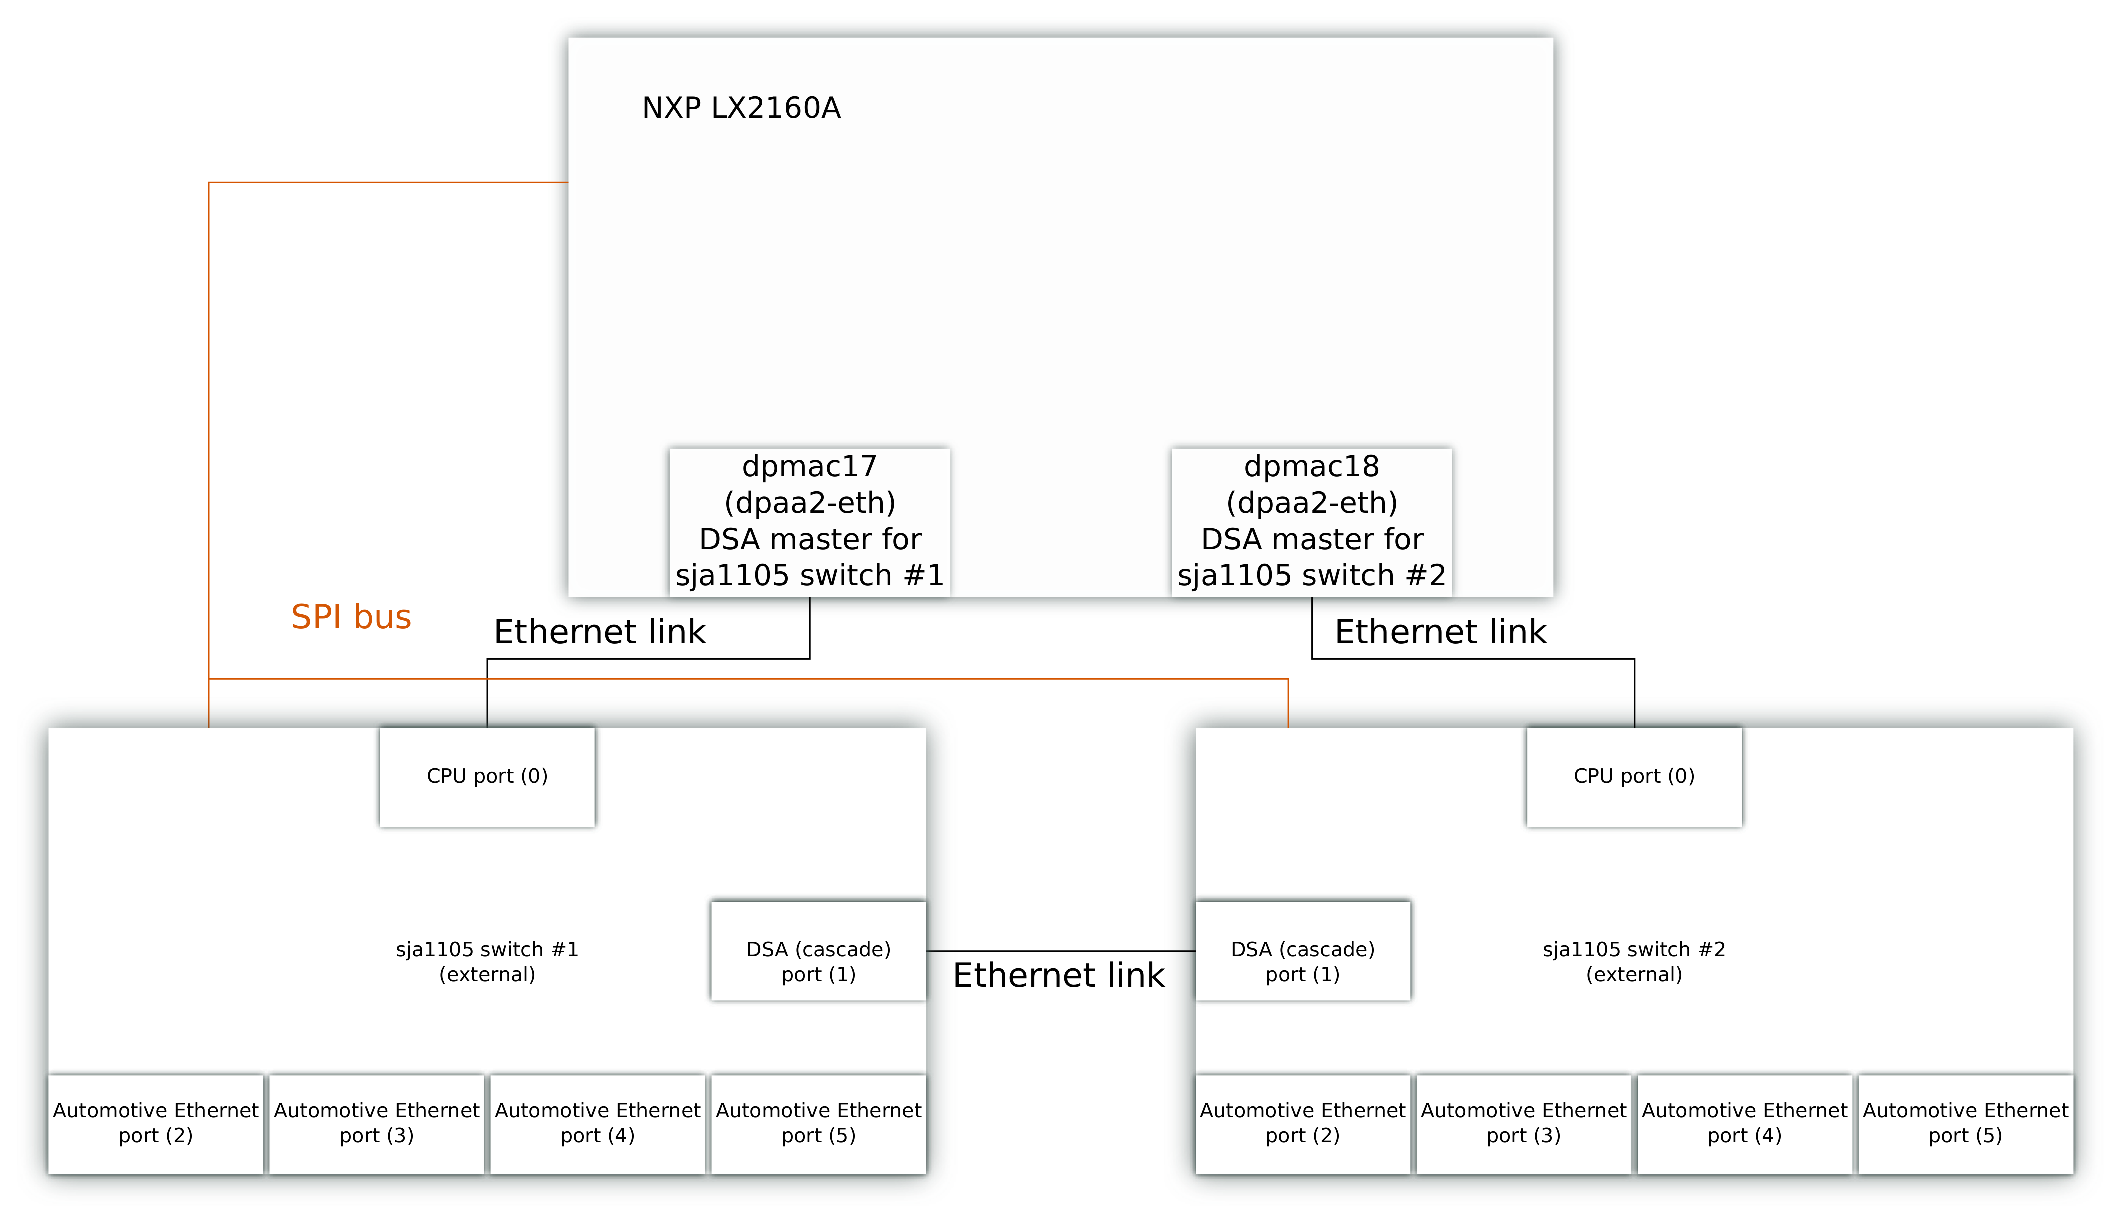
\includegraphics[width=\columnwidth]{nxp-bluebox3-h-tree.eps}
  \caption{A H-tree topology consisting of two switches, each having its own CPU port, but also a cascade port for autonomous forwarding towards the other switch}
  \label{nxp-bluebox3-h-tree}
\end{figure}

The second is the H tree topology \cite{dsa-h-tree}, described by figure
\ref{nxp-bluebox3-h-tree}. In such a system, there are multiple switches
laterally interconnected through cascade ports, but to reach the CPU, each
switch has its own dedicated CPU port. It turns out that to support such a
system, there are two distinct issues.

First, with regard to RX filtering, an H tree topology is very similar in
challenges to a single switch with multiple CPU ports. Hardware address
learning on the CPU port, if at all available, is of no use and leads to
addresses bouncing and packet drops. All MAC addresses which need to be
filtered to the host need to be installed on all CPU ports as static FDB
entries. This has led to the extension of the bridge switchdev FDB notifiers to
cover FDB entries that are local to the bridge, and which should not be
forwarded.

Secondly, in an H topology it is actually possible to have packet loops with
the TX forwarding offload feature enabled, because TX data plane packets sent
by the stack to one switch might also be flooded through the cascade port to
the other switch, where they might be again flooded to the second switch's CPU
port, where they will be processed as RX packets. Currently, drivers which
support this topology need to be individually patched to cut RX from cascade
ports that go towards switches that have their own CPU port, because the DSA
driver API does not have the necessary insight into driver internals as to be
able to cut forwarding between two ports only in a specific direction.

\section{Future changes}

One of the most important features still absent from DSA is the support for
multiple CPU ports. However, with many roadblocks such as basic RX filtering
support now out of the way, this functionality will arrive sooner rather than
later. A possible implementation of multiple CPU ports should follow several
requirements.

First of all, when there are multiple CPU ports there are multiple DSA masters,
and DSA has gained the ability for the tagging protocol to be changed at
runtime, by writing the new tagging protocol's name into the \verb|dsa/tagging|
sysfs file of the DSA master. But since both DSA masters attach to the same DSA
tree, asymmetric DSA tagging protocols should not be permitted; all DSA masters
should use the same protocol, since this might have undesirable effects for
other switches in the same tree.

DSA should preserve its current default configuration, meaning that it should
not use multiple CPU ports by default, but pick the first CPU port and keep the
other one as inactive.

At the very least, user space should be able to create a static assignment
between a user port and the DSA master interface that services it, using a
rtnetlink attribute. Device tree descriptions are not welcome since they should
only describe the hardware ability, not the configuration. Furthermore, the
kernel should provide the means but not enforce the policy.

Configuring the CPU ports in a link aggregation group is also a common use
case which should be permitted by the design. While the network is down, the
DSA masters can be added by user space to a bonding or team interface, and DSA
ports can be statically assigned to use that bonding interface as the DSA master.
Transmission from software towards the switch is balanced in software, while
transmission from the switch towards the CPU is balanced by a hardware LAG that
is the mirror image of the bonding interface.

There is also the emerging topic of Ethernet controllers as DSA masters that
are aware of the DSA switches beneath them, which is typical when both the
switch and the Ethernet controller are made by the same silicon vendor.
Right now DSA can freely inherit all \verb|master->vlan_features|, such as TX
checksumming offloads, but this does not work for all switch and DSA master
combinations, so it must be refined and only the known-working master and
switch combinations inherit the extra features.

On the same topic of DSA-aware masters, SR-IOV capable masters are expected to
still work when attached to a DSA switch, but the network stack's model of this
use case is unclear. VFs on top of a DSA master should be treated as switched
endpoints, but the VF driver's transmit and receive procedures do not go
through the DSA tagging protocol hooks, and these packets are therefore
DSA-untagged. So hardware manufacturers have the option of inserting DSA tags
in hardware for packets sent through a VF that goes through a DSA switch. It is
unclear, however, according to which bridging domain are these VFs being
forwarded. An effort should be made to standardize the way in which the network
stack treats these interfaces. It appears reasonable that DSA switches might
have to register virtual network interfaces that are facing each VF of the
master, in order to enforce their bridging domain, but this makes the DSA
master and switch drivers closely coupled.

On the other hand, letting other code paths than the DSA tagging protocol
driver inject packets into the switch risks compromising the integrity of the
hardware, which is an issue that currently exists and needs to be addressed.

\section{The case for network interfaces for the CPU ports}

The DSA architecture mandates that ports which are unable of terminating
traffic in a meaningful way do not get network interfaces associated with them.
One example is the CPU port: attempting to ping on the interface associated
with that would mean that a packet is sent towards the inside of the system, in
a loopback of sorts.

On the other hand, there has always been the argument of needing network
interfaces associated with the shared (CPU and DSA) ports for the ability to
retrieve statistics counters, which are a very useful debugging tool. The
latter argument could not win over the former, and other techniques for
debugging the DSA shared ports have been developed: devlink port regions,
devlink resources, as well as overlaying the ethtool statistics counters of the
CPU port on top of the statistics counters of the DSA master.

Additionally, the PHY library needed a network interface attached to the PHY,
and while the link between the DSA master and the switch is typically a fixed
set of traces on a PCB, that is not always the case. For example, a Raspberry
Pi might connect using a plain RJ45 cable to a switch evaluation board. In that
case, there are two Ethernet PHYs involved between the DSA master and the
switch, and the PHY library must manage them. To solve that scenario, the PHY
library and phylink have been modified to be able to instantiate the state
machines in lack of an attached network interface, and still present the same
API towards the MAC side \cite{dsa-cpu-port-phylink}.

There have also been attempts to register network interfaces for the CPU ports
in order to offload tc shapers on them, to limit the amount of traffic sent to
the host \cite{dsa-tc-cpu-port}. These attempts have been shot down due to the
impracticality of installing an egress shaper as opposed to an ingress policer
on the front-facing ports directly. With an egress shaper, packets would be
eventually dropped due to congestion. With an ingress policer, they would be
dropped early when the bandwidth quota is exceeded.

So the architecture has remained unchanged despite the temptations. However,
there might be use cases where network interfaces for the CPU port make the
most amount of sense. Detailed below is one such example, which is provided for
the purpose of contemplating the idea, the usage model for this new interface,
and other consequences. Note that creating a network interface for the CPU port
does not imply that interfaces are created for cascade ports too, so the
aforementioned use cases for a network interface for hidden ports should still
search for an alternative.

The Time Sensitive Networking (TSN) enhancements to IEEE 802.1Q and IEEE 802.3
are aiming to transform Ethernet into a viable replacement for the existing
buses in automotive and industrial networking, and are seeing hardware
implementations in a number of recently added DSA switch drivers. In TSN, the
real-time guarantees are obtained by enforcing bandwidth reservations and
saying "no" when those reservations are exceeded. Packets with real-time
guarantees must be able to be transported by the same network that transports
best-effort traffic, and time division based access to the network is therefore
a common approach. To minimize the latency, the real-time aware endpoints must
be synchronized to the network time via the Precision Time Protocol (PTP), in
order to always send and receive packets in band with their alloted time
interval, and not have switches delay their packets until that interval comes.

One of the existing paradigms in TSN is the "switched endpoint", a mix between
an application terminating some data in a time-synchronized manner, and a
control stack for the on-board switch, which forwards the data that must not be
terminated locally. At the bare minimum, the switch control stack must manage a
port redundancy protocol and the synchronization protocol.

Such use cases are well suited for a DSA hardware design, since the endpoint
can be a real-time application which opens a socket on the DSA master, and the
switch can be managed by DSA itself.

There are multiple reasons why a TSN endpoint application might want to run on
the bare DSA master. First, the switch might simply have a "lightly managed"
design, and it might accept DSA-untagged packets just fine.

Second, opening the socket on top of the bridge interface, or on top of the
switch interfaces, would add the extra processing overhead of several virtual
network interfaces in the kernel, which would cost a few precious tens of extra
microseconds per packet. DSA and the Linux bridge are simply not optimized for
packet latency.

Third, the DSA master might be well prepared for TSN offloads itself, not
relying on the TSN offloads of the switch. The DSA master might itself be
synchronized to the PTP time, it might have a time-aware packet scheduler
configured (standardized as clause "8.6.8.4 Enhancements for scheduled traffic"
of IEEE 802.1Q-2018, but widely known as IEEE 802.1Qbv).  Also, the endpoint
application might want to be as oblivious to the network topology as possible,
it should not need to know which switch port interface to bind its socket to,
binding to the DSA master should be sufficiently agnostic if the CPU port is
viewed as a regular bridged port.

In this model, it would make perfect sense for the CPU port to have a network
interface associated with it. This interface would be capable of traffic, and
pinging on the CPU port would talk to an application doing the same thing but
running on the DSA master. Putting the CPU port interface in a bridge would
decide what happens to DSA-untagged packets sent by the bare DSA master. It
would not affect in any way what happens with control or data packets injected
by DSA on behalf of the switch network interfaces or on behalf of a bridge, and
packets belonging to those flows would still reach the CPU port even if that
port was not under a bridge, or the same bridge. In this model, the DSA master
could also be an endpoint (a DSA-unaware one), and the CPU port interface would
be the bridge port that services it.

Nonetheless, there are many reasons why the switched endpoint use case cannot
be realized with the existing DSA infrastructure today.

\begin{itemize}
\item Having the DSA master synchronized to the PTP time means running two
      instances of the PTP state machine on the same system: one for the DSA
      master, as an endpoint (Ordinary Clock), and one for the switch
      interfaces, as a bridge (Boundary Clock). Since the DSA master and the
      DSA switch have independent PTP Hardware Clocks (PHC), the DSA master's
      PHC will synchronize itself to the switch's PHC. Due to limitations in
      the PTP user API, DSA disables PTP timestamping on the master interface
      \cite{deny-ptp-on-dsa-master}. The PTP user space API would need to be
      extended, and timestamps to be annotated with the interface/PHC that took
      them, before the DSA master and the switch could synchronize themselves.
\item On TX, it has been established in the sections above that letting DSA
      unaware code paths simply inject packets at will into the switch can be
      a harmful operation. If crafted correctly, packets sent from outside
      DSA-controlled code paths can even modify state inside the switch (access
      registers, etc). It would be desirable that if switch drivers create a
      path for DSA-untagged packet flows coming from the DSA master, those
      paths are safe.
\item On RX, DSA traps all packets received by the DSA master by default. But
      allowing a packet reception flow outside of DSA's control would mean that
      the tagging protocol driver needs to filter out the packets that must be
      processed by the DSA master itself, and not by the DSA switch interfaces.
      As opposed to the TX flow, where packets coming from the DSA code paths
      will be DSA-tagged and packets coming from DSA-unaware code paths will be
      DSA-untagged, the same expectation is unreasonable for RX, unless the
      switch knows beforehand somehow that some packets sent towards the CPU
      must be tagged, and some must not. So the filtering, as well as tag
      stripping decision, must take place in software, inside the DSA tagging
      protocol driver. The criterion by which the tagging protocol decides what
      packets should be stripped and then left in the hands of the DSA master
      is TBD, but could possibly be derived from the source and destination MAC
      addresses of the packet (the DSA master as a switched endpoint would need
      to have a different MAC address than the virtual switch interfaces).
\end{itemize}

While the above might sound like fiction, the NXP LS1028A SoC targets the above
use cases, but the DSA framework's restrictions were avoided by using a special
hardware design. Namely, the internal switch present inside this SoC has two
CPU ports, but they are asymmetric in role. One internal switch port can act as
a control port (and the associated ENETC port is the DSA master), while the
other port is a plain data port, for which DSA registers a user port with a
network interface, and for which the associated ENETC port is not a DSA master.
This can be seen in figure \ref{nxp-ls1028a-control-data-ports}.

\begin{figure}[ht]
  \centering
  \includegraphics[width=\columnwidth]{nxp-ls1028a-control-data-ports.eps}
  \caption{NXP LS1028A control port and data port}
  \label{nxp-ls1028a-control-data-ports}
\end{figure}

Both switch ports 4 and 5 are CPU ports in the truest sense of the word: they
are inwards-facing ports that lead to the CPU. However, from DSA's perspective
they play very different roles. The ENETC has its own PHC, and the Felix switch
has its own PHC, and when the control port is physically separate from the data
port, synchronizing the two is not any more complicated than running:

\begin{verbatim}
# ptp4l -i eno2 -2 -P -m &
# ptp4l -i swp4 -2 -P -m &
\end{verbatim}

Since switch port 4 can be configured by software to act as either as a control
or a data port, and the same goes for switch port 5, the device tree
description becomes challenging. It is desirable in many use cases that the
device tree is no more than a description of the hardware, since it may be set
in stone with no way of updating it in the field. But when port roles are
customizable, it is tempting to make that customization in the device tree
description itself.

In mainline Linux, the NXP LS1028A has only one internal switch port described
as a CPU port (has an \verb|ethernet| phandle to its ENETC pair). The other
internal switch port is declared as a simple data port, or disabled.

But the \verb|ethernet| phandle might have been just as well between
\verb|mscc_felix_port5| and \verb|enetc_port3|. Additionally, the felix driver
might gain support for multiple CPU ports when using the \verb|ocelot-8021q|
tagging protocol, and it is desirable that both ports are described as CPU
ports in the device tree when that happens, but also that this does not break
existing use cases when using the normal \verb|ocelot| DSA tagging protocol.

It would therefore appear natural for the device tree to describe a port's
capability of acting as a control interface, and the definitive device tree
description for the LS1028A switch to have the \verb|ethernet| properties on
both CPU ports. But the DSA framework could also ask the driver if it wants to
opt in to registering a network interface for CPU ports.
In the case of the Ocelot switch family, which the LS1028A Felix switch is a
part of, DSA-untagged packets received on the control port are not accepted, so
this driver would refuse that feature. However, in the presence of multiple
\verb|ethernet| OF properties, DSA currently picks the first one as the CPU
port, and leaves the other ports with this property as CPU ports too, but they
are "inactive" CPU ports (no \verb|dp->cpu_dp| pointer points to them). It
would be for this "inactive" CPU port that the DSA framework can register a
network interface, and this would effectively yield the same result as the
current description where one of the internal switch ports is declared as a
user port.

Moreover, the data port opt-in might have uses beyond the LS1028A.
Fundamentally, the aforementioned "switched endpoint" use case is the same as
the LS1028A's use of two internal ports, except that the packet flows for the
control and data ports are overlaid on top of a single pair of hardware ports.
When the DSA switch is external, it might be wasteful to connect two Ethernet
ports to the system in this way just for them to play different roles.

Even with a dedicated control port and a dedicated control port, the NXP
LS1028A workaround still has some limitations. It creates a separate hardware
path for DSA untagged packets to exit the system, but this path does not scale.
To explain this, we can return to the example switch topology with disjoint
trees, only this time, inside the LS1028A, both \verb|eno2| and \verb|eno3|
ports are enabled. This is shown in figure \ref{felix-sja1105-with-eno2-as-data-port}.

\begin{figure}[ht]
  \centering
  \includegraphics[width=\columnwidth]{felix-sja1105-with-eno2-as-data-port}
  \caption{The same disjoint tree setup with felix and sja1105, but with eno2 as a data port}
  \label{felix-sja1105-with-eno2-as-data-port}
\end{figure}

DSA-untagged packets can exit the internal Felix switch, but attached to the
Felix switch are other DSA switches that expect packets to be tagged with their
own switch-specific DSA tag. So these packets will be going nowhere, unless we
accept one of the following:

\begin{itemize}
\item Similar to SR-IOV network interfaces which are DSA-aware and can be
      configured to insert a certain programmable DSA header in hardware, it is
      sane for DSA switch hardware designs to be themselves DSA-aware, and to
      insert other switch's tag formats on egress. In this case, the Felix
      switch would need to insert a DSA tag compatible with the sja1105's
      expectations, to allow DSA-untagged packets coming from eno2 to exit.
\item The need for a path for DSA-untagged packets coming from inside the
      system to exit the switch is acknowledged at the DSA framework level, and
      does not need workarounds such as multiple CPU ports with different
      roles. Such a path for DSA-untagged packets can then be added to the
      drivers of the downstream switches too, and packets coming from eno2 can
      be treated as DSA-untagged all the way down.
\end{itemize}

At a minimum, exposing a network interface for the switch CPU port would allow
the PTP protocol to run between the switch and the DSA master, and would allow
the user to control the forwarding path for DSA-untagged traffic coming from
the master or other upstream interfaces. And the reverse: any attempt to expose
interfaces for the hidden ports needs to answer what are their semantics in
terms of packet I/O, considering that "no packet I/O" is not a viable option.

\section{Conclusion}

This paper attempts to describe the considerations and angles that should be
taken into account when writing DSA switch drivers, or when extending the DSA
framework. In some cases the requirements are contradictory, and writing a DSA
driver can be more of a creative process than an objective one with a clear
goal.

Taming DSA switches and making them behave completely in accordance with the
network stack's expectations proves to be a much more ambitious challenge than
initially foreseen, thus the fight continues.

\newpage

\begin{minipage}{\textwidth}
\begin{thebibliography}{2}

\bibitem{dsa-netdev-2.1}
Distributed Switch Architecture, A.K.A. DSA\\
\url{https://legacy.netdevconf.info/2.1/papers/distributed-switch-architecture.pdf}

\bibitem{reject-dsa-masters-as-bridge-ports}
net: bridge: reject DSA-enabled master netdevices as bridge members\\
\url{https://git.kernel.org/pub/scm/linux/kernel/git/netdev/net-next.git/commit/?id=8db0a2ee2c6302a1dcbcdb93cb731dfc6c0cdb5e}

\bibitem{dsa-disjoint-trees}
[v4,resend,net-next,0/4] Cross-chip bridging for disjoint DSA trees\\
\url{http://patchwork.ozlabs.org/project/netdev/cover/20200510163743.18032-1-olteanv@gmail.com/}

\bibitem{dsa-h-tree}
[v3,net-next,0/8] NXP SJA1105 driver support for "H" switch topologies\\
\url{https://patchwork.kernel.org/project/netdevbpf/cover/20210804135436.1741856-1-vladimir.oltean@nxp.com/}

\bibitem{dsa-hsr}
[net-next,v3,0/4] add HSR offloading support for DSA switches\\
\url{https://patchwork.kernel.org/project/netdevbpf/cover/20210210010213.27553-1-george.mccollister@gmail.com/}

\bibitem{dsa-lag}
[v5,net-next,0/5] net: dsa: Link aggregation support\\
\url{https://patchwork.kernel.org/project/netdevbpf/cover/20210113084255.22675-1-tobias@waldekranz.com/}

\bibitem{switchdev-explicit-offloading-api}
[v6,net-next,0/7] Let switchdev drivers offload and unoffload bridge ports at their own convenience\\
\url{https://patchwork.kernel.org/project/netdevbpf/cover/20210721162403.1988814-1-vladimir.oltean@nxp.com/}

\bibitem{bridge-tx-fwd-offload}
Merge branch 'bridge-tx-fwd'\\
\url{https://git.kernel.org/pub/scm/linux/kernel/git/netdev/net-next.git/commit/?id=356ae88f8322066a2cd1aee831b7fb768ff2905c}

\bibitem{switchdev-fdb-on-foreign-interfaces}
net: dsa: listen for SWITCHDEV\_{FDB,DEL}\_ADD\_TO\_DEVICE on foreign bridge neighbors\\
\url{https://git.kernel.org/pub/scm/linux/kernel/git/netdev/net-next.git/commit/?id=d5f19486cee79d04c054427577ac96ed123706db}

\bibitem{dsa-assisted-learning}
Merge branch 'offload-software-learnt-bridge-addresses-to-dsa'\\
\url{https://git.kernel.org/pub/scm/linux/kernel/git/netdev/net-next.git/commit/?id=c214cc3aa8423ba8e67c7028eeea9b0f48e8a7e6}

\bibitem{dsa-rx-filtering}
Merge branch 'dsa-rx-filtering'\\
\url{https://git.kernel.org/pub/scm/linux/kernel/git/netdev/net-next.git/commit/?id=7f4e5c5b8cb00138ad1a10cab87bbd1e2d4d3376}

\bibitem{deny-ptp-on-dsa-master}
net: dsa: Deny PTP on master if switch supports it\\
\url{https://git.kernel.org/pub/scm/linux/kernel/git/netdev/net-next.git/commit/?id=f685e609a301f171b62ee52a69acc3a74c2c04aa}

\bibitem{dsa-cpu-port-phylink}
[v2,net-next,00/11] Decoupling PHYLINK from struct net\_device\\
\url{http://patchwork.ozlabs.org/project/netdev/cover/1559065097-31832-1-git-send-email-ioana.ciornei@nxp.com/}

\bibitem{dsa-tc-cpu-port}
dsa traffic priorization\\
\url{https://lore.kernel.org/netdev/20190918140225.imqchybuf3cnknob@pengutronix.de/}

\end{thebibliography}
\end{minipage}

\end{document}
https://git.kernel.org/pub/scm/linux/kernel/git/netdev/net-next.git/commit/?id=edac6f6332d96aab59af5f27a195f55cd080f034
